Lately, improving electricity use in homes is becoming more and more critical. Enhancing electricity usage is possible through the \textit{Demand Response} algorithm that allows users to manage their energy consumption correctly, reply better to peak demand or electricity market offers and utilise the energy resources more efficiently.\\
This work intends proposes an hour-ahead Demand Response algorithm for Home Energy Management System (HEMS) that uses machine learning techniques, considering electricity costs and client's dissatisfaction. \\
Specifically, because of the inherent nature in hour-ahead electricity price market, the customer accesses only one price for the current hour. To deal with the uncertainty in future prices, a stable price forecasting model is presented, which is implemented by a Long Short-Term Memory (LSTM). It is a particular Recurrent Neural Network capable of learning long-term dependencies.\\
Price's prediction has become an essential argument in today's electrical engineering, and numerous methods have been tested for its implementation. The LSTM method is easy and efficient to implement, showing good predictions due to the nature of the prices: a time series strictly correlated. \\
Fig. \ref{fig:HEMS} shows the detailed DR algorithm that combines the long short-term memory and multi-agent reinforcement learning. Every hour, the HEMS receives the hour-ahead price, and uses the LSTM to predict the future prices (twelve hours forecasted). In cooperation with the forecasted future prices, MARL is adopted to make optimal decisions for different appliances in a decentralized manner, to minimize the user energy bill and degree of discomfort. Here, each appliance has an agent, and RL is used for decision-making in the context of uncertainty regarding the price information and load demand of the appliances.

\begin{figure}[h]
    \centering
    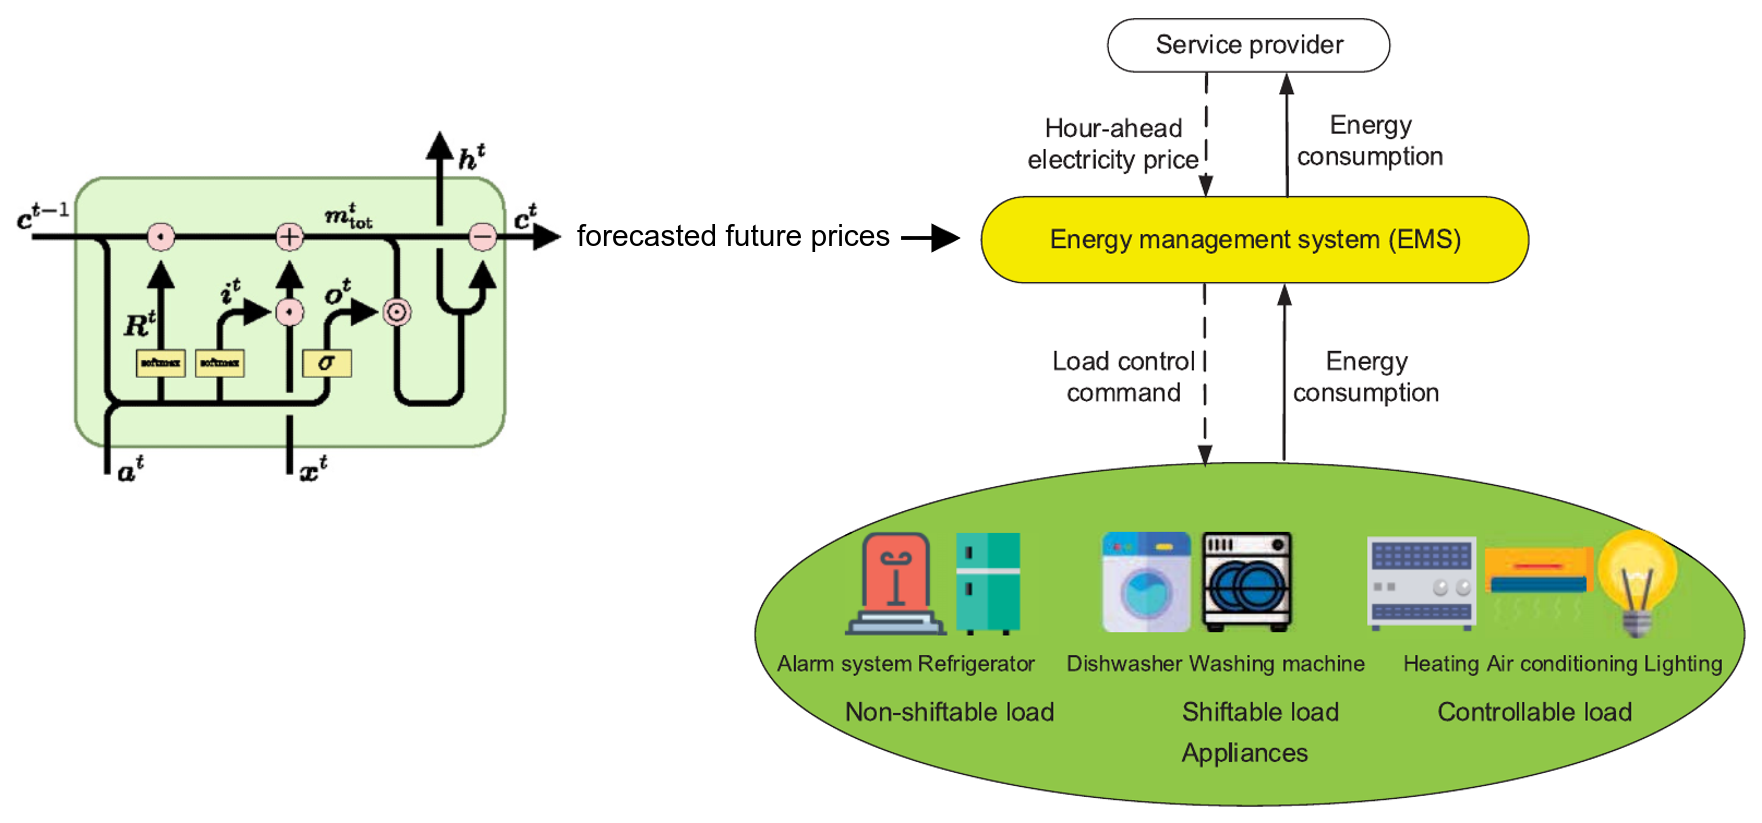
\includegraphics[width=\textwidth]{HEMS.png}
    \caption{HEMS architecture}
    \label{fig:HEMS}
\end{figure}